\documentclass{beamer}
%
% Choose how your presentation looks.
%
% For more themes, color themes and font themes, see:
% http://deic.uab.es/~iblanes/beamer_gallery/index_by_theme.html
%
\mode<presentation>
{
  \usetheme{Warsaw}      % or try Darmstadt, Madrid, Warsaw, ...
  \usecolortheme{seahorse} % or try albatross, beaver, crane, ...
  \usefonttheme{serif}  % or try serif, structurebold, ...
  \setbeamertemplate{navigation symbols}{}
  \setbeamertemplate{caption}[numbered]
} 

\usepackage[english]{babel}
\usepackage[utf8x]{inputenc}

\title{Graph Isomorphism Problem}
\subtitle{with programming project focused on Tree Isomorphism Problem}
\author{Kamil Szymon Jadeszko}
\institute{HS Mittweida \\ Network Algorithms Course}
\date{January 11th, 2016}

\usepackage[english]{babel}
\usepackage[utf8x]{inputenc}
\usepackage{graphicx}
\usepackage{adjustbox}
\usepackage{amsmath}
\usepackage{amssymb}
\usepackage{amsthm}
\usepackage{caption}
\usepackage{float}
\usepackage{wasysym}
\usepackage{mathtools}

\usepackage{algorithm2e}
\usepackage{algorithmic}
\usepackage{float}

\newtheorem{thm}{Theorem}[section]
\newtheorem{rem}[thm]{Remarks}
\newtheorem{lem}[thm]{Lemma}
\newtheorem{ex}[thm]{Example}

\begin{document}

\begin{frame}
  \titlepage
\end{frame}

% Uncomment these lines for an automatically generated outline.
%\begin{frame}{Outline}
%  \tableofcontents
%\end{frame}

\section{About Graph Isomorphism}

\begin{frame}

\begin{definition}[Graph Isomorphism]
Let $G_1 = (V_1, E_1)$ and $G_2 = (V_2, E_2)$ be graphs.  \\
	A mapping $\phi : V_1 \rightarrow V_2$ is called \alert{graph isomorphism} iff $$\forall u,v \in V_1 ~~~~ (u,v) \in E_1 \iff (\phi(u),\phi(v)) \in E_2 . $$
\end{definition}

\begin{block}{Remark}
If this mapping exists we say that \alert{ $G_1$ and $G_2$ are isomorphic}.  
\end{block}
\end{frame}

\begin{frame}

\begin{block}{Examples}
[on the board]
\end{block}

\end{frame}


\begin{frame}

\begin{itemize}
\item GIP is NP problem. 
\pause
\item There is still open question if GIP is NP-complete problem. 
\pause
\item Brute force algorithm has complexity $O(n!)$
\pause
\item Best known algorithm runs in $2^{O(\log^c(n))}$ time - very new boundary, work of László Babai, published last year. Previous $2^{O(\sqrt{n\log(n)})}$
\pause
\item GIP has practical applications - biology, cryptography, 
\end{itemize}

\end{frame}

\section{About Tree Isomorphism}

\begin{frame}{It's not so easy to live with computer scientists}

% Commands to include a figure:
\begin{figure}
	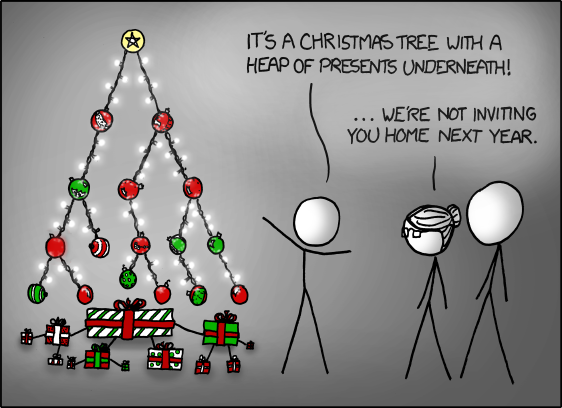
\includegraphics[scale=0.5]{img1}
	\caption{\label{fig:your-figure} source: XKCD.com}
\end{figure}

\end{frame}


\begin{frame}
\begin{definition}[Tree]
	\alert{Tree} is  simple, connected, acyclic graph.
\end{definition}
\end{frame}

\begin{frame}
\begin{definition}[Rooted tree]
	\alert{Rooted tree $T(V,E,r)$}  is  a tree with one selected vertex $r \in V$ called root.
\end{definition}
\end{frame}


\begin{frame}{Did I told you, that computer scientists are weird?}

% Commands to include a figure:
\begin{figure}
	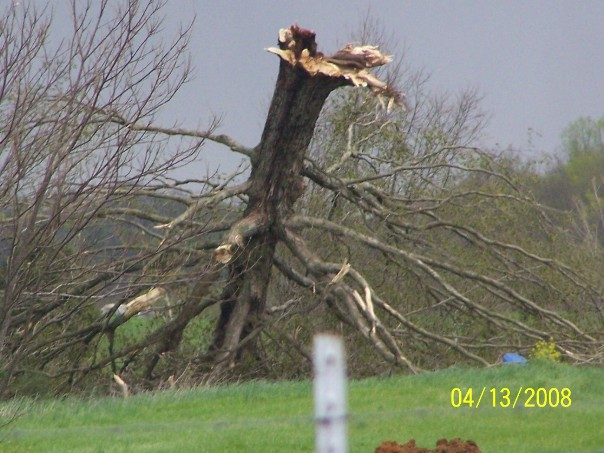
\includegraphics[scale=1]{img2}
	\caption{\label{fig:your-figure} source: weather.gov}
\end{figure}
\end{frame}

\begin{frame}
Basic terms:
	\begin{enumerate}
      \item Root
      \item Leaf
      \item Child
    \end{enumerate}
\end{frame}


\begin{frame}{Python project}
	\begin{enumerate}
      \item Rooted Ordered Trees
      \item Rooted Trees
      \item Ordinary Trees
    \end{enumerate}
\end{frame}

\begin{frame}{Specific case - ordered (planted) trees}

\begin{definition}[first() and next() operator]
[on the board]
\end{definition}
\begin{definition}[Rooted Ordered Tree Isomorphism]
\small
Let $T_1 = (V_1,E_1, r_1)$ and $T_2 = (V_2,E_2, r_2) $ be two ordered trees. \\
Mapping $\phi : V_1 \rightarrow V_2$ is called \alert{ordered tree isomorphism} iff:
\begin{enumerate}
\item $\phi(r_1) = r_2$
\item $\phi(first(v)) = first(\phi(v))$ ~ for all $v \in V_1$ where $v$ isn't a leaf
\item $\phi(next(v)) = next(\phi(v))$ ~ for all $v \in V_1$ where $v$ is nonlast child 
\end{enumerate}
\end{definition}
\end{frame}



\begin{frame}{Algorithm (ROTI)}
	\begin{enumerate}
    \item Compare trees sizes - if are different trees aren't isomorphic.
	\item Assign to every vertex of $T_1$ his index in pre-order traversal.
    \item Assign to every vertex of $T_2$ his index in pre-order traversal.
    \item Make bijection $\phi : V_1 \rightarrow V_2$ s.t $$\phi(v_1) = v_2  \iff index(v_1) = index(v_2)$$
    \item Check previous mentioned conditions of r.o.t. isomorphism for $\phi$ 
    \end{enumerate}
\end{frame}

\begin{frame}{Algorithm}
\begin{block}{Complexity}
	This algorithm runs in $O(n)$ time, where n is size of tree.
\end{block}
\end{frame}


\begin{frame}{Rooted trees}
\begin{definition}[Rooted Tree Isomorphism]
Let $T_1 = (V_1, E_1, r_1)$ and $T_2 = (V_2, E_2, r_2)$ be rooted trees  \\
	A mapping $\phi : V_1 \rightarrow V_2$ is called \alert{rooted tree isomorphism} iff $$\phi \text{ is graph isomorphism ~~~~and} ~~~~ \phi(r_1) = r_2$$
\end{definition}
\begin{block}{Examples}
[on the board]
\end{block}

\end{frame}


\begin{frame}{Algorithm (Rooted tree labeling)}
	[explanation using interactive python shell]
\end{frame}


\begin{frame}{Algorithm (RTI)}
	\begin{enumerate}
    \item Compare trees sizes - if they are different trees aren't isomorphic.
    \item Compare labels of trees - if they are different trees aren't isomorphic, otherwise - they are. 
    \end{enumerate}
\end{frame}

\begin{frame}{Algorithm}
\begin{block}{Complexity}
	This algorithm runs in $O(n^2 \cdot \log(n))$ time, where n is size of tree and can be easy optimized to $O(n^2)$
\end{block}

\begin{block}{Remark}
	There exist rooted tree isomorphism algorithms which run in $O(n)$ and can be found in positions 1. and 2. from references.
\end{block}

\end{frame}

\begin{frame}{Ordinary trees}
  \begin{enumerate}
    \item Naive way. 
    \item Better way.
  \end{enumerate}
\end{frame}


\begin{frame}{Ordinary trees}

\begin{block}{Lemma}
Existence of $O(n)$-complexity algorithm for rooted tree implies existence of $O(n)$-complexity algorithm for ordinary trees.
\end{block}

Proof:  [on the board]
\begin{definition}[Tree center]
A \alert{center of tree} is a vertex $v$ such that the longest path from $v$ to a leaf is minimal over all vertices.
\end{definition}

\end{frame}


\begin{frame}
		\begin{center}	
			 Thank you for your attention.
		\end{center} 
\end{frame}
 


\begin{frame}{References}


\begin{thebibliography}{1}
\beamertemplatebookbibitems
\bibitem{H} A. Aho, J. Hopcrot, J. Ullman
			\newblock \emph{The Design and Analysis of Computer Algorithms} 
\bibitem{V} G. Valiente
			\newblock\emph{Algorithms on Trees and Graphs}


\beamertemplatearticlebibitems
\bibitem{B} M. Bonamy
			\newblock\emph{A Small Report on Graph and Tree Isomorphism} 
\bibitem{B} A. Smal
			\newblock\emph{Tree Isomorphism Talk} 
            
 	
\end{thebibliography}

\end{frame}






\end{document}
